\documentclass[12pt]{book}

\usepackage{titlesec}
\usepackage{setspace}
\usepackage[a4paper,margin=2cm]{geometry}
\usepackage[export]{adjustbox}
\usepackage{amsmath}
\usepackage{amssymb,amsfonts}
\usepackage{color,xcolor,graphicx,multicol,multirow,booktabs,url,subfig,lastpage}
\usepackage{pstricks,pst-sigsys,pst-circ,pst-plot,pst-eucl,pstricks-add}
\usepackage{float}
\usepackage{comment}
\usepackage{enumerate}
\usepackage{ragged2e}
\usepackage{eso-pic}
\usepackage{standalone}
\usepackage{autonum}
\usepackage{todonotes}

     
\numberwithin{equation}{section}
\numberwithin{figure}{section}
\numberwithin{table}{section}

% Header and footer.
\usepackage{fancyhdr}
\pagestyle{fancy}
\fancyhf{}
\setlength{\headheight}{2cm}
\setlength{\textheight}{23cm}
\fancyhead[C]{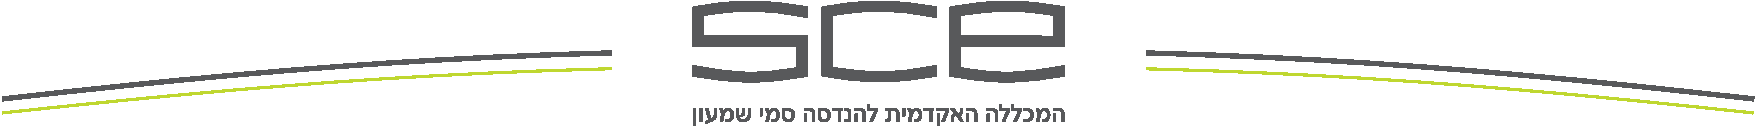
\includegraphics[width=\linewidth]{header}}
%\fancyfoot[C]{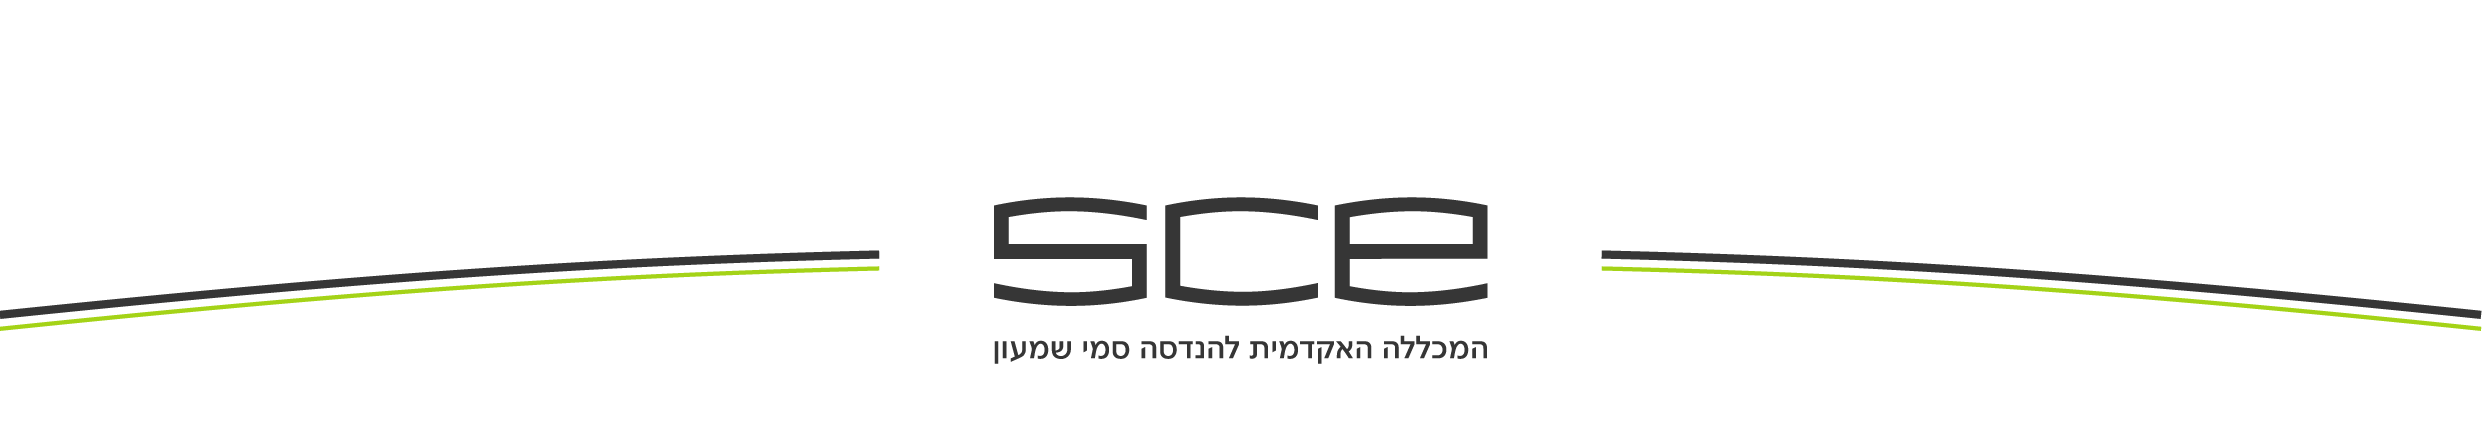
\includegraphics[width=0.5\linewidth]{footer}}
\renewcommand{\headrulewidth}{0cm}


%Hebrew and english.
\usepackage{mathspec}
\usepackage{polyglossia}
% OVERLEAF SETTING
\usepackage{fontspec}
\setotherlanguage[calendar=hebrew, numerals=arabic]{hebrew}
\setdefaultlanguage{english}
\newfontfamily\hebrewfont{David CLM}
\let\hebrewfonttt\ttfamily
% LOCAL SETTING
%\setdefaultlanguage[calendar=hebrew, numerals=arabic]{hebrew}
%\setotherlanguage{english}
%\newfontfamily\hebrewfont{Arial}
%\setmainfont{Arial}
%\setmonofont{Courier New}

%  \makeatletter
%  \renewcommand{\thesection}{\arabic{section}\@SepMark\thechapter} % if using book class
%  \renewcommand{\thesubsection}{\arabic{subsection}\@SepMark\arabic{section}\@SepMark\thechapter}
% \renewcommand{\thesubsubsection}{\arabic{subsubsection}\@SepMark\thesubsection}
%  \renewcommand{\thefigure}{\arabic{figure}\@SepMark\thechapter}
%  \makeatother

% \makeatletter
% \renewcommand{\SepMark}[1]{\def\@SepMark{#1}}
% \makeatother
% \SepMark{.}
 
%  \makeatletter
%  \def\maketag@@@#1{\hbox{\m@th\normalfont\LRE{#1}}} %\LRE
%  \def\tagform@#1{\maketag@@@{(\ignorespaces#1\unskip)}}
%  \makeatother



%Equation numbring correction.
% \makeatletter
% \def\maketag@@@#1{\hbox{\m@th\normalfont\LRE{#1}}}
% \def\tagform@#1{\maketag@@@{(\ignorespaces#1\unskip)}}
% \makeatother


\newcommand*{\mypstrickspic}[1]{%
 \IfFileExists{./#1.pdf}%
 {\includegraphics{./#1.pdf}}%
 {\input{./#1.tex}}%
}


\begin{document}
\begin{hebrew}
\vspace*{0.1cm}
\begin{center}
\fontsize{16pt}{19pt}
\selectfont

{\Large   שם הפרויקט}
\vspace*{0.5cm}

{\Large פרויקט הנדסי}

\vspace*{1cm}

\fontsize{14pt}{17pt}
\selectfont

\textbf{דו''ח מכין / דו''ח מסכם}
\vspace*{1.5cm}

\fontsize{10pt}{12pt}
\selectfont

הוכן לשם מילוי דרישות חלקיות לקבלת

תואר ראשון בהנדסה \LR{B. Sc}

\vspace*{1cm}

מאת

\vspace*{1cm}

\fontsize{16pt}{19pt}
\selectfont

{\Large שם סטודנט 1}

\vspace*{0.5cm}

{\Large שם סטודנט 2}

\fontsize{12pt}{12pt}
\selectfont

\vspace*{1cm}

בהנחיית תואר ושם מנחה

\vspace*{2cm}

\fontsize{14pt}{17pt}
\selectfont

\textbf{הוגש למחלקה להנדסת חשמל ואלקטרוניקה}
  
\textbf{המכללה האקדמית להנדסה אשדוד}

\vspace*{3cm}

\begin{english}\today\end{english} ~~~~~~~~~~~~~~~~~~~~~~~~~~~~~\Hebrewtoday


\end{center}

\newpage

\vspace*{0.1cm}
\begin{center}
\fontsize{16pt}{19pt}
\selectfont

{\Large שם הפרויקט}
\vspace*{0.5cm}

{\Large פרויקט הנדסי}

\vspace*{1cm}

\fontsize{14pt}{17pt}
\selectfont

\textbf{דו''ח מכין / דו''ח מסכם}
\vspace*{1.5cm}

\fontsize{10pt}{12pt}
\selectfont

הוכן לשם מילוי דרישות חלקיות לקבלת

תואר ראשון בהנדסה \LR{B. Sc}

\vspace*{1cm}

מאת

\vspace*{1cm}

\fontsize{16pt}{19pt}
\selectfont

{\Large שם סטודנט 1}

\vspace*{0.5cm}

{\Large שם סטודנט 2}

\fontsize{12pt}{12pt}
\selectfont

\vspace*{1cm}

בהנחיית תואר ושם מנחה

\vspace*{2cm}

\fontsize{14pt}{17pt}
\selectfont

\textbf{הוגש למחלקה להנדסת חשמל ואלקטרוניקה}
  
\textbf{המכללה האקדמית להנדסה אשדוד}

\vspace*{3cm}
\end{center}

\fontsize{10pt}{12pt}
\selectfont

חתימת הסטודנט: \rule{3cm}{1pt} ~~~~~~~~~תאריך: \rule{3cm}{1pt}

\vspace*{0.5cm}

חתימת המנחה: \rule{3cm}{1pt} ~~~~~~~~~~~~תאריך: \rule{3cm}{1pt}

\vspace*{0.5cm}

אישור ועדת הפרויקטים: \rule{2cm}{1pt} ~~~~~~~~~תאריך: \rule{3cm}{1pt}




\newpage
\doublespacing


\fontsize{12pt}{15pt}
\selectfont

עמוד אופציונלי -  הפרויקט ההנדסי נעשה בשיתוף עם שם החברה/מפעל

בהנחיית תוארו המקצועי ושם המנחה הנוסף – אם קיים

\newpage


יש להכניס את העמוד בספר הסופי בלבד.

\vspace*{1cm}

תחום הפרויקט:   מערכות הספק – תקשורת – RF – אלקטרואופטיקה – לווינים –

\vspace*{1cm}

 סוג הפרויקט:   מחקרי - מעשי

 \vspace*{1cm}

\LR{Keywords: .........................}

\vspace*{1cm}

מילות מפתח: ...................

\vspace*{1cm}

יש לבחור לפחות 2 מילות מפתח מבין אלה רשומות מטה:

מיקרומחשבים, מעגלים אלקטרוניים \LR{ (Microelectronics)}

מערכות הספק \LR{(Power Systems)}

מערכות בקרה \LR{ (Control Systems)}

\LR{RF (Radiofrequency) }

עיבוד אותות \LR{(Signal Processing)}

עיבוד תמונות ווידאו \LR{(Image and Video Processing)}

מערכות הספק אלקטרוניות \LR{(Electronic Power Systems, Power Electronics)}

חיישנים ומכשור \LR{(Sensors and Instrumentation)}

תקשורת \LR{(Communications)}

אלקטרואופטיקה ותקשורת אופטית \LR{(Optoelectronics and Optic Communications)}

לייזרים ויישומיהם \LR{(LASERs and applications)}

לייזרים ברפואה \LR{(LASERs and medicine)}

תקשורת לוויינית \LR{(Satellite Communications)}

מערכות מגנטיות, שדות \LR{(Magnetic Systems)}

הינע חשמלי \LR{(Electrical Drive)}

מערכות בדיקה \LR{(Verification and Test  Systems)}

מיקרוגלים \LR{(Microwaves)}

אנטנות \LR{(Antennas)}

רובוטיקה \LR{(Robotics)}

מערכות מתח גבוה \LR{(High voltage systems)}

\newpage

\section*{הבעת תודה}
\addcontentsline{toc}{chapter}{\numberline{}הבעת תודה}

ברצוני להביע את תודתי ל-...


\newpage

\section*{\centering \begin{hebrew} תקציר \end{hebrew}}
\addcontentsline{toc}{chapter}{\numberline{}תקציר}

כתוב את תקצירך כאן

\end{hebrew}
\newpage

\section*{\centering Abstract}
\addcontentsline{toc}{chapter}{\numberline{}Abstract}
\LR{
COPY YOUR ENGLISH ABSTRACT HERE
}

% == table of contents, list of figures and tables. ==
\cleardoublepage
\tableofcontents
\cleardoublepage
\listoffigures
%\addcontentsline{toc}{chapter}{\numberline{}רשימת האיורים}
\cleardoublepage
\listoftables
%\addcontentsline{toc}{chapter}{\numberline{}רשימת הטבלאות}
\cleardoublepage


\newpage
\setcounter{page}{1}
\pagenumbering{arabic}
\newpage

\renewcommand{\baselinestretch}{2}


% Introduction
\setcounter{chapter}{1}
\section*{\centering Chapter 1 - Introduction}
\addcontentsline{toc}{chapter}{\numberline{} Chapter 1 - Introduction}

%%% Local Variables:
%%% mode: latex
%%% TeX-master: "template_english"
%%% End:

% Survey
\newpage
\setcounter{chapter}{2}
\section*{\centering Chapter 2 - Literature Survey}
\addcontentsline{toc}{chapter}{\numberline{} Chapter 2 - Literature Survey}

\section{Deep Learning}

\section{Boum}

%%% Local Variables:
%%% mode: latex
%%% TeX-master: "template_english"
%%% End:

% Your Solution
\newpage
\setcounter{chapter}{3}
\section*{\centering Chapter 3 - Proposed Solution}
\addcontentsline{toc}{chapter}{\numberline{} Chapter 3 - Proposed Solution}

%%% Local Variables:
%%% mode: latex
%%% TeX-master: "template_english"
%%% End:

% Results
\newpage
\setcounter{chapter}{4}
\section*{\centering Chapter 4 - Results and Discussion}
\addcontentsline{toc}{chapter}{\numberline{}  Chapter 4 - Results and Discussion}

%%% Local Variables:
%%% mode: latex
%%% TeX-master: "template_english"
%%% End:

\newpage

\section*{\centering Chapter 5 - Conclusion and perspectives}
\addcontentsline{toc}{chapter}{\numberline{} Chapter 5 - Conclusion and perspectives}

Write here conclusions and perspectives

\newpage

% ================== רשימת מקורות ====================

\section*{\centering References}
\addcontentsline{toc}{chapter}{\numberline{} References}
%\printbibliography

\bibliographystyle{IEEEtran}
\bibliography{myBib}




\newpage

\renewcommand{\thepage}{A-\arabic{page}}
\setcounter{page}{1}
\section*{\centering Appendix}
\addcontentsline{toc}{chapter}{\numberline{} Appendix}

\section*{Appendix A}
\addcontentsline{toc}{section}{\numberline{} Appendix A}

\begin{hebrew}
מפאת המספר הרב של הפונקציות וקבצי המטלב הקשורים לפרויקט, הועלו כל הקבצים הנחוצים להתבוננות בשלבי הפרויקט לתיקייה הניתנת לגישה בלינק הבא: 

\url{https://drive.google.com/open?id=xxxxxxxx}

להקלת הניווט, פתח את קובץ הטקסט המכיל הסברים הודות הקבצים.

\end{hebrew}





\end{document}


%%% Local Variables:
%%% mode: latex
%%% TeX-master: t
%%% End:
